\section{Water Channel Subsystem (WCS)}%
\label{sec:wcs}

Il WCS gestisce l'attuatore e l'interfaccia operatore locale.
Riceve dal CUS lo stato del sistema e il comando di apertura della valvola, aggiornando di conseguenza il servomotore e il display LCD.
Attraverso pulsante e potenziometro consente inoltre all'operatore di inviare richieste al CUS, senza modificare autonomamente lo stato globale.

\subsection{Architettura e hardware}
Il WCS è implementato su Arduino UNO con firmware C++ basato sul framework Arduino.
La classe \code{HWPlatform} gestisce l'accesso ai dispositivi hardware, mentre \code{Context} mantiene l'ultimo stato ricevuto dal CUS, comprendente modalità operativa, apertura comandata e disponibilità dello stato.

I collegamenti dei componenti sono riportati nella Tabella~\ref{tab:wcs-pins} e rappresentati nello schema della Figura~\ref{fig:wcs-wiring}.

\begin{table}[htbp]
\centering
\begin{tabularx}{\linewidth}{@{}l X@{}}
\toprule
\textbf{Pin} & \textbf{Componente e funzione} \\
\midrule
D8 & Pulsante con circuito RC per attenuare i rimbalzi del segnale. \\
A0 & Ingresso analogico del potenziometro. \\
D9 & Segnale di controllo del servomotore. \\
A4 / A5 & Collegamenti SDA / SCL del display LCD I2C. \\
USB & Comunicazione seriale con il CUS a 115200 baud. \\
\bottomrule
\end{tabularx}
\caption{Collegamenti hardware del WCS.}%
\label{tab:wcs-pins}
\end{table}

\begin{figure}[htbp]
\centering
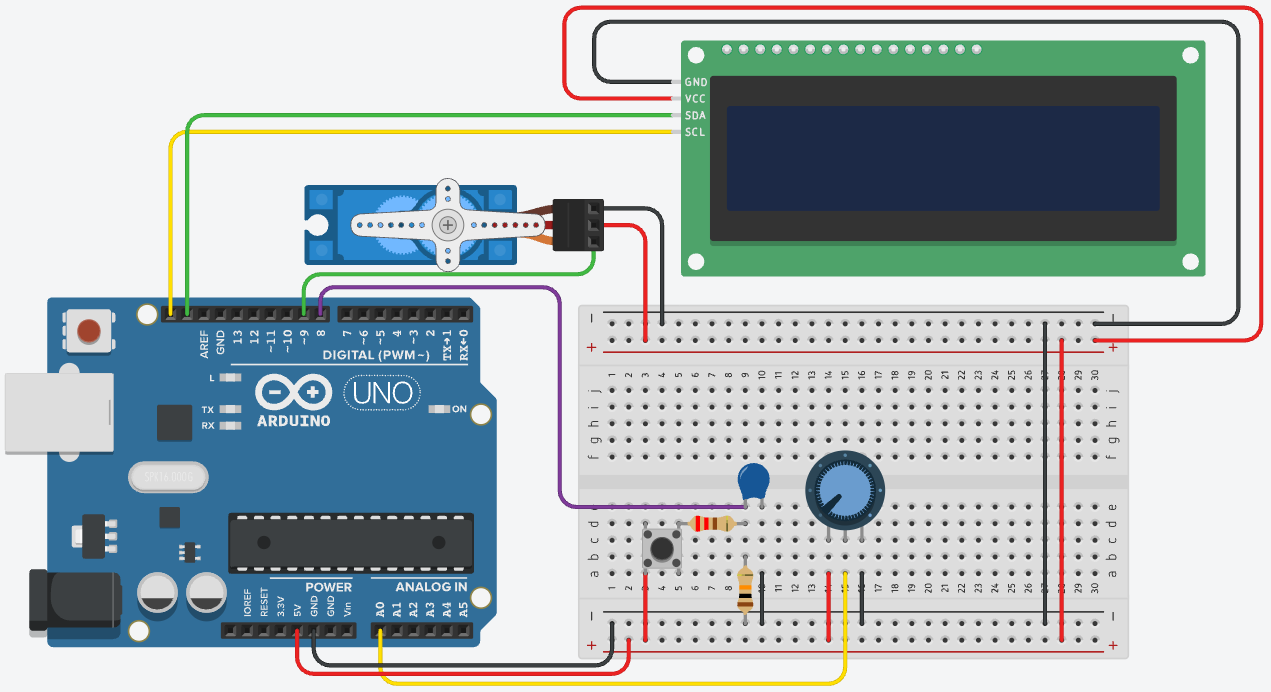
\includegraphics[width=0.96\linewidth]{figures/wcs_wiring.png}
\caption{Schema dei collegamenti del prototipo WCS realizzato con Tinkercad.}%
\label{fig:wcs-wiring}
\end{figure}

\FloatBarrier%

\subsection{Scheduler, task e macchine a stati}
Il firmware è organizzato in task, ciascuno dedicato a una specifica funzione del WCS.
La loro esecuzione è gestita da uno scheduler cooperativo, che li richiama in sequenza secondo i rispettivi periodi.
Timer1 fornisce il riferimento temporale con un intervallo di base di \(50\,\mathrm{ms}\).

I task, le rispettive responsabilità e i periodi di esecuzione sono riportati nella Tabella~\ref{tab:wcs-tasks}.


\begin{table}[htbp]
\centering
\begin{tabularx}{\linewidth}{@{}l c X@{}}
\toprule
\textbf{Task} & \textbf{Periodo} & \textbf{Responsabilità} \\
\midrule
SerialCommTask & 50 ms &
Gestione della comunicazione seriale con il CUS. \\

ButtonTask & 50 ms &
Rilevamento delle pressioni e richieste di cambio modalità. \\

PotentiometerTask & 100 ms &
Lettura del potenziometro e richieste di apertura. \\

ValveTask & 50 ms &
Aggiornamento del servomotore. \\

DisplayTask & 200 ms &
Aggiornamento delle informazioni sul display LCD. \\
\bottomrule
\end{tabularx}
\caption{Task del WCS e relativi periodi di esecuzione.}%
\label{tab:wcs-tasks}
\end{table}

I task condividono il \code{Context}, che contiene lo stato ricevuto dal CUS.
Timer1 è dedicato allo scheduler, mentre Timer2 viene utilizzato dalla libreria \code{ServoTimer2} per il controllo del servomotore.

La gestione del pulsante e del potenziometro è organizzata attraverso due FSM, rappresentate nella Figura~\ref{fig:wcs-fsms}.

\begin{figure}[htbp]
\centering

\begin{tikzpicture}[node distance=3.2cm and 3cm]

\node[state] (released) {RELEASED};
\node[state,right=of released] (pressed) {PRESSED};

\draw[flow] (released) to[bend left=22]
    node[above,font=\footnotesize,align=center]
    {pressione / richiesta} (pressed);

\draw[flow] (pressed) to[bend left=22]
    node[below,font=\footnotesize]
    {rilascio} (released);

\node[state,below=of released] (disabled) {DISABLED};
\node[state,right=of disabled] (active) {ACTIVE};

\draw[flow] (disabled) to[bend left=22]
    node[above,font=\footnotesize,align=center]
    {MANUAL confermato /\\ acquisizione riferimento} (active);

\draw[flow] (active) to[bend left=22]
    node[below,font=\footnotesize]
    {uscita da MANUAL} (disabled);

\end{tikzpicture}

\par\smallskip

\begin{minipage}{0.94\linewidth}
\footnotesize
\raggedright%

\textbf{Condizioni operative:}

\begin{itemize}
    \setlength{\itemsep}{2pt}
    \setlength{\parsep}{0pt}
    \setlength{\topsep}{3pt}

    \item \textbf{Pulsante:}
    una richiesta per pressione, senza ripetizioni fino al rilascio.

    \item \textbf{Potenziometro:}
    in ACTIVE invia una richiesta per variazioni di almeno 5 punti percentuali o al raggiungimento di un estremo con variazione non nulla.

    \item \textbf{Stati iniziali:}
    RELEASED e DISABLED.
\end{itemize}

\end{minipage}

\caption{Macchine a stati per la gestione del pulsante e del potenziometro.}%
\label{fig:wcs-fsms}
\end{figure}

\code{ButtonTask} distingue gli stati \code{RELEASED} e \code{PRESSED}, generando una richiesta al rilevamento della pressione.
Il circuito RC attenua i rimbalzi del pulsante, mentre la FSM evita richieste ripetute finché il segnale rimane attivo.
Prima della sincronizzazione con il CUS e durante \code{UNCONNECTED}, i comandi locali sono disabilitati.

\code{PotentiometerTask} opera invece negli stati \code{DISABLED} e \code{ACTIVE}.
Quando il CUS conferma l'ingresso in \code{MANUAL}, il task acquisisce la posizione corrente del potenziometro come riferimento, senza inviare immediatamente un comando.

Le successive variazioni della manopola generano richieste di apertura quando raggiungono una soglia minima di spostamento.
Sono inoltre gestiti gli estremi di apertura, per consentire il raggiungimento completo dello \(0\%\) e del \(100\%\).

\FloatBarrier%


\subsection{Interfaccia operatore e controllo della valvola}%
\label{subsec:wcs-interface}

All'avvio il WCS mantiene il servomotore in posizione di chiusura e il display mostra un messaggio di attesa.
Prima di rendere operativi i controlli locali, il sistema si sincronizza con il CUS e acquisisce uno stato valido.

Il pulsante permette di richiedere il cambio tra le modalità \code{AUTOMATIC} e \code{MANUAL}.
In modalità \code{MANUAL}, il potenziometro consente di richiedere una diversa apertura della valvola.

Le richieste vengono inviate al CUS, che ne determina l'accettazione.
Il WCS aggiorna servomotore e display soltanto in base allo stato successivamente ricevuto, mantenendo il controllo centralizzato del sistema.

Il task \code{ValveTask} converte la percentuale di apertura comandata, compresa tra \(0\%\) e \(100\%\), in un angolo di comando del servomotore tra \(0^\circ\) e \(90^\circ\).

Il display LCD mostra la modalità operativa e la percentuale di apertura della valvola.
Le informazioni vengono aggiornate quando cambia lo stato ricevuto.


\subsection{Validazione e limitazioni}

Le prove funzionali sul prototipo hanno confermato il comportamento dei controlli locali, dell'attuatore, del display e della comunicazione con il CUS.

Il WCS non dispone di un feedback sulla posizione effettiva del servomotore e non gestisce automaticamente il ripristino delle interruzioni della comunicazione seriale.
